% Graphic for TeX using PGF
% Title: /tmp/Diagram1.dia
% Creator: Dia v0.95
% CreationDate: Sun Oct 25 14:07:46 2009
% For: kapranov
% \usepackage{tikz}
% The following commands are not supported in PSTricks at present
% We define them conditionally, so when they are implemented,
% this pgf file will use them.
\ifx\du\undefined
  \newlength{\du}
\fi
\setlength{\du}{15\unitlength}
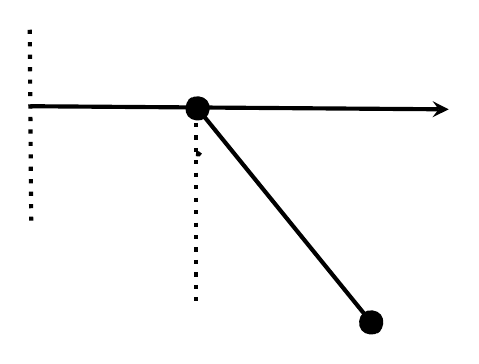
\begin{tikzpicture}
\pgftransformxscale{1.000000}
\pgftransformyscale{-1.000000}
\definecolor{dialinecolor}{rgb}{0.000000, 0.000000, 0.000000}
\pgfsetstrokecolor{dialinecolor}
\definecolor{dialinecolor}{rgb}{1.000000, 1.000000, 1.000000}
\pgfsetfillcolor{dialinecolor}
\pgfsetlinewidth{0.100000\du}
\pgfsetdash{}{0pt}
\pgfsetdash{}{0pt}
\pgfsetbuttcap
{
\definecolor{dialinecolor}{rgb}{0.000000, 0.000000, 0.000000}
\pgfsetfillcolor{dialinecolor}
% was here!!!
\pgfsetarrowsend{stealth}
\definecolor{dialinecolor}{rgb}{0.000000, 0.000000, 0.000000}
\pgfsetstrokecolor{dialinecolor}
\draw (4.974783\du,2.074756\du)--(15.050000\du,2.150000\du);
}
\pgfsetlinewidth{0.100000\du}
\pgfsetdash{{\pgflinewidth}{0.200000\du}}{0cm}
\pgfsetdash{{\pgflinewidth}{0.200000\du}}{0cm}
\pgfsetbuttcap
{
\definecolor{dialinecolor}{rgb}{0.000000, 0.000000, 0.000000}
\pgfsetfillcolor{dialinecolor}
% was here!!!
\definecolor{dialinecolor}{rgb}{0.000000, 0.000000, 0.000000}
\pgfsetstrokecolor{dialinecolor}
\draw (8.952879\du,2.177243\du)--(8.952879\du,6.914858\du);
}
\pgfsetlinewidth{0.100000\du}
\pgfsetdash{}{0pt}
\pgfsetdash{}{0pt}
\pgfsetbuttcap
{
\definecolor{dialinecolor}{rgb}{0.000000, 0.000000, 0.000000}
\pgfsetfillcolor{dialinecolor}
% was here!!!
\definecolor{dialinecolor}{rgb}{0.000000, 0.000000, 0.000000}
\pgfsetstrokecolor{dialinecolor}
\pgfpathmoveto{\pgfpoint{8.962106\du}{3.228484\du}}
\pgfpatharc{124}{11}{0.456626\du/0.456626\du}
\pgfusepath{stroke}
}
\pgfsetlinewidth{0.100000\du}
\pgfsetdash{{\pgflinewidth}{0.200000\du}}{0cm}
\pgfsetdash{{\pgflinewidth}{0.200000\du}}{0cm}
\pgfsetbuttcap
{
\definecolor{dialinecolor}{rgb}{0.000000, 0.000000, 0.000000}
\pgfsetfillcolor{dialinecolor}
% was here!!!
\definecolor{dialinecolor}{rgb}{0.000000, 0.000000, 0.000000}
\pgfsetstrokecolor{dialinecolor}
\draw (4.957726\du,0.232699\du)--(4.993081\du,4.899604\du);
}
\pgfsetlinewidth{0.100000\du}
\pgfsetdash{}{0pt}
\pgfsetdash{}{0pt}
\pgfsetbuttcap
{
\definecolor{dialinecolor}{rgb}{0.000000, 0.000000, 0.000000}
\pgfsetfillcolor{dialinecolor}
% was here!!!
}
\definecolor{dialinecolor}{rgb}{0.000000, 0.000000, 0.000000}
\pgfsetstrokecolor{dialinecolor}
\draw (8.811458\du,1.894400\du)--(13.372296\du,7.515899\du);
\pgfsetlinewidth{0.100000\du}
\pgfsetdash{}{0pt}
\pgfsetmiterjoin
\pgfsetbuttcap
\definecolor{dialinecolor}{rgb}{0.000000, 0.000000, 0.000000}
\pgfsetfillcolor{dialinecolor}
\pgfpathmoveto{\pgfpoint{8.811458\du}{1.894400\du}}
\pgfpathcurveto{\pgfpoint{8.927942\du}{1.799894\du}}{\pgfpoint{9.138932\du}{1.821872\du}}{\pgfpoint{9.233438\du}{1.938356\du}}
\pgfpathcurveto{\pgfpoint{9.327944\du}{2.054841\du}}{\pgfpoint{9.305966\du}{2.265831\du}}{\pgfpoint{9.189482\du}{2.360337\du}}
\pgfpathcurveto{\pgfpoint{9.072998\du}{2.454843\du}}{\pgfpoint{8.862007\du}{2.432865\du}}{\pgfpoint{8.767501\du}{2.316381\du}}
\pgfpathcurveto{\pgfpoint{8.672995\du}{2.199897\du}}{\pgfpoint{8.694973\du}{1.988906\du}}{\pgfpoint{8.811458\du}{1.894400\du}}
\pgfusepath{fill}
\pgfsetlinewidth{0.100000\du}
\pgfsetdash{}{0pt}
\pgfsetmiterjoin
\pgfsetbuttcap
\definecolor{dialinecolor}{rgb}{0.000000, 0.000000, 0.000000}
\pgfsetfillcolor{dialinecolor}
\pgfpathmoveto{\pgfpoint{13.372296\du}{7.515899\du}}
\pgfpathcurveto{\pgfpoint{13.255812\du}{7.610405\du}}{\pgfpoint{13.044822\du}{7.588427\du}}{\pgfpoint{12.950315\du}{7.471943\du}}
\pgfpathcurveto{\pgfpoint{12.855809\du}{7.355458\du}}{\pgfpoint{12.877787\du}{7.144468\du}}{\pgfpoint{12.994272\du}{7.049962\du}}
\pgfpathcurveto{\pgfpoint{13.110756\du}{6.955456\du}}{\pgfpoint{13.321746\du}{6.977434\du}}{\pgfpoint{13.416253\du}{7.093918\du}}
\pgfpathcurveto{\pgfpoint{13.510759\du}{7.210402\du}}{\pgfpoint{13.488781\du}{7.421393\du}}{\pgfpoint{13.372296\du}{7.515899\du}}
\pgfusepath{fill}
\end{tikzpicture}
